\documentclass[11pt,a4paper]{article}

% ------------------------------------------------------------------
% LogicWard — Design & Engineering Specification
% Compile:  pdflatex (run twice for TOC/refs)  or  latexmk -pdf
% ------------------------------------------------------------------

\usepackage[utf8]{inputenc}
\usepackage[T1]{fontenc}
\usepackage{lmodern}
\usepackage[margin=2.2cm]{geometry}
\usepackage[dvipsnames,table]{xcolor}
\usepackage{booktabs}
\usepackage{tabularx}
\usepackage{longtable}
\usepackage{array}
\usepackage{listings}
\usepackage{titlesec}
\usepackage{enumitem}
\usepackage{fancyhdr}
\setlength{\headheight}{24pt}
\addtolength{\topmargin}{-10pt}
\usepackage{parskip}
\usepackage[most]{tcolorbox}
\usepackage{tikz}
\usetikzlibrary{arrows.meta,positioning,shapes.geometric,backgrounds,fit}
\usepackage{underscore}
\usepackage[hidelinks]{hyperref}

% ---------------- palette (Prahari-derived) ----------------
\definecolor{navy}{HTML}{14304F}
\definecolor{navy2}{HTML}{1D4370}
\definecolor{accent}{HTML}{3987E5}
\definecolor{ink}{HTML}{1F2937}
\definecolor{muted}{HTML}{5B6B80}
\definecolor{good}{HTML}{0E7A0E}
\definecolor{warn}{HTML}{A16207}
\definecolor{serious}{HTML}{C05621}
\definecolor{critical}{HTML}{C02626}
\definecolor{page}{HTML}{EEF0F4}
\definecolor{hair}{HTML}{DBE0E8}
\definecolor{codebg}{HTML}{F6F8FB}

\hypersetup{colorlinks=true,linkcolor=navy2,urlcolor=accent}

% ---------------- headings ----------------
\titleformat{\section}{\Large\bfseries\color{navy}}{\thesection}{0.6em}{}
\titleformat{\subsection}{\large\bfseries\color{navy2}}{\thesubsection}{0.6em}{}
\titleformat{\subsubsection}{\normalsize\bfseries\color{ink}}{\thesubsubsection}{0.6em}{}
\titlespacing*{\section}{0pt}{1.4em}{0.6em}

% ---------------- header / footer ----------------
\pagestyle{fancy}
\fancyhf{}
\renewcommand{\headrulewidth}{0.4pt}
\renewcommand{\headrule}{\hbox to\headwidth{\color{hair}\leaders\hrule height \headrulewidth\hfill}}
\fancyhead[L]{\small\color{muted}\textbf{LogicWard}\,\textbullet\, OT Drift-Detection Appliance}
\fancyhead[R]{\small\color{muted}Design Spec v1.1}
\fancyfoot[C]{\small\color{muted}\thepage}

% ---------------- code listings ----------------
\lstdefinestyle{lw}{
  basicstyle=\ttfamily\small\color{ink},
  backgroundcolor=\color{codebg},
  frame=single,
  framesep=6pt,
  rulecolor=\color{hair},
  breaklines=true,
  columns=fullflexible,
  keepspaces=true,
  showstringspaces=false,
  xleftmargin=4pt,
  xrightmargin=4pt,
  aboveskip=8pt,belowskip=8pt,
}
\lstset{style=lw}

% ---------------- callout boxes ----------------
\newtcolorbox{keybox}[1][]{colback=accent!6,colframe=accent,boxrule=0.8pt,
  left=8pt,right=8pt,top=6pt,bottom=6pt,arc=2pt,#1}
\newtcolorbox{warnbox}[1][]{colback=critical!5,colframe=critical,boxrule=0.8pt,
  left=8pt,right=8pt,top=6pt,bottom=6pt,arc=2pt,#1}

\newcommand{\code}[1]{\texttt{\small #1}}
\newcolumntype{L}{>{\raggedright\arraybackslash}X}

% ==================================================================
\begin{document}

% ---------------- title page ----------------
\begin{titlepage}
\thispagestyle{empty}
\vspace*{1.2cm}
{\color{navy}\rule{\textwidth}{2.5pt}}\\[0.5cm]
{\Huge\bfseries\color{navy} LogicWard}\\[0.35cm]
{\LARGE\color{navy2} Live OT Drift-Detection Appliance}\\[0.5cm]
{\large\color{ink} Detect unauthorized PLC logic changes on a thermal power plant\\ before they become operational risk.}\\[0.3cm]
{\color{navy}\rule{\textwidth}{2.5pt}}\\[1.2cm]

\begin{tcolorbox}[colback=page,colframe=hair,boxrule=1pt,arc=3pt]
\large
\textbf{Document:} Design \& Engineering Specification \\[4pt]
\textbf{Version:} 1.1 (as built) \hfill \textbf{Date:} 2026-07-28 \\[4pt]
\textbf{Status:} Built \& verified --- 98/98 automated checks across 7 suites \\[4pt]
\textbf{Audience:} Engineering team \& collaborating agents
\end{tcolorbox}

\vspace{1cm}
{\large\bfseries\color{navy2} At a glance}
\begin{itemize}[leftmargin=1.4em,itemsep=3pt]
  \item A Raspberry Pi is the PLC (Modbus TCP) for a simulated thermal power plant.
  \item A second machine is the attacker; a laptop runs the detection engine + SOC dashboard.
  \item One event contract; three detection planes (cyber, physical, resource) on one bus.
  \item Rungs are \emph{data} to baseline and diff --- \textbf{no ladder-logic interpreter}.
  \item Reuses three existing repos: OT\_SECURITY, PiSentinel, and Prahari.
\end{itemize}

\vfill
{\small\color{muted} Built for a cybersecurity hackathon. Reuses and re-themes prior work:
OT\_SECURITY (Modbus server + attacker), PiSentinel (dashboard + network/resource sensors),
Prahari (scoring, demo choreography, SOC design language).}
\end{titlepage}

\tableofcontents
\newpage

% ==================================================================
\section{Executive summary}

\textbf{LogicWard} is a live Operational-Technology (OT) security appliance that continuously
verifies a Programmable Logic Controller (PLC) against a \textbf{cryptographically hashed,
approved baseline} and raises severity-ranked, MITRE-mapped alerts the instant the running logic
or process state drifts from that baseline.

The demonstration models a \textbf{thermal power plant}. A \textbf{Raspberry Pi} acts as the PLC,
running a Modbus TCP server plus a thin edge sensor agent. A \textbf{second machine} acts as the
attacker. A \textbf{laptop} runs the detection engine and a professional Flask dashboard with
role-based access control.

\begin{keybox}
\textbf{Core insight.} A PLC ``program'' is \emph{data}, not something we execute. LogicWard does
\emph{not} build a ladder-logic interpreter. It treats the approved rung set as structured data to
baseline, and treats the PLC's live Modbus registers as ground-truth reality. Detection is a
continuous \textbf{diff} of live-vs-baseline across two surfaces: the structural program and the
live register state.
\end{keybox}

Everything speaks \textbf{one event contract}. Three detection planes (cyber, physical, resource)
all emit the same \code{Event} object onto a single \textbf{event bus}, which enriches each event
with attacker identity and a MITRE ATT\&CK for ICS technique, appends it to a tamper-evident
evidence log, and streams it to the dashboard.

\subsection{What a judge sees in 8 minutes}
\begin{enumerate}[leftmargin=1.5em,itemsep=2pt]
  \item A quiet, professional SOC dashboard showing a live thermal plant running normally.
  \item An attacker on a second machine drifts the PLC --- changing a safety setpoint, inverting
        trip logic, injecting a rogue rung, hijacking an output coil.
  \item LogicWard lights up in real time: a side-by-side baseline-vs-current diff with the exact
        changes highlighted, a severity-ranked alert feed, each alert mapped to a named MITRE
        ATT\&CK for ICS technique.
  \item Physical-tampering and resource-exhaustion (DDoS) attacks are caught by the same fabric.
  \item One click exports a signed PDF forensic report: who, when, what changed, and the ICS
        technique used.
\end{enumerate}

% ==================================================================
\section{Implementation update (v1.1 --- as built \& verified)}

\begin{keybox}
The system is \textbf{built and passing 98 automated checks across 7 test suites}.
Three v1.0 decisions were upgraded; this section is the authoritative delta ---
read it alongside the original sections that follow.
\end{keybox}

\subsection{Changed from the v1.0 draft}
\begin{itemize}[leftmargin=1.4em,itemsep=3pt]
  \item \textbf{Program format is real Rockwell L5X XML, not JSON.} The program is a
    genuine \code{.L5X} export; the engine parses it with \code{lxml},
    \textbf{canonicalizes} it (strips volatile ExportDate/EditedDate/revisions/CRC and
    non-logic comments) and diffs canonical rung structure. A date-only re-export or a
    comment edit yields an \emph{identical} structural hash (no false positives); an
    operator flip / setpoint drift / coil hijack changes it. Neutral-text ladder is
    parsed into instruction/operand structs so all six mutations are still named.
  \item \textbf{Baseline lock is HMAC-SHA256 signed} (\code{engine/baseline.py}); editing
    the locked baseline on disk breaks the signature. Integrity, not access control.
  \item \textbf{Passive FIM via \code{watchdog}} watches \textbf{both} files: the Pi's
    running \code{live.L5X} (out-of-band tamper $\rightarrow$ \code{cyber.program\_file\_modified})
    and the laptop's signed baseline (change $\rightarrow$ HMAC re-verify $\rightarrow$
    \code{cyber.baseline\_tamper} critical, or \code{cyber.baseline\_relocked} info).
  \item \textbf{GitHub-style side-by-side diff} (\code{engine/l5x\_diff.py}, \code{difflib}):
    the dashboard highlights baseline-vs-live rungs with row- and word-level red/green.
  \item \textbf{SIEM-ready JSONL} --- already satisfied by the evidence log.
  \item \textbf{Docker: deliberately not included} (hardware-coupled Pi sensors + live-demo
    robustness).
\end{itemize}

\subsection{Verification (98/98) and how to run}
\begin{tabularx}{\textwidth}{@{}l r L@{}}
\toprule
\textbf{Suite} & \textbf{Checks} & \textbf{Covers} \\
\midrule
\code{smoke\_bus} & 15/15 & event bus, ingest/poll, forwarder, MITRE, evidence \\
\code{smoke\_l5x} & 16/16 & L5X parse + canonicalize; no-false-positive; real changes \\
\code{smoke\_plant} & 14/14 & thermal Modbus reads; setpoint write fires a trip; program endpoints \\
\code{smoke\_drift} & 18/18 & HMAC lock/tamper; all 6 mutations w/ severity+MITRE+channel \\
\code{smoke\_agent} & 10/10 & sensors (sim) + real watchdog FIM + agent$\rightarrow$ingest wiring \\
\code{smoke\_dashboard} & 15/15 & login/RBAC, drift surfacing, diff API, PDF, actions \\
\code{smoke\_attacker} & 10/10 & every attack drives the expected detection end-to-end \\
\bottomrule
\end{tabularx}

\smallskip
\textbf{Run:} dashboard \code{python -m logicward.dashboard.app} (login \code{soc/soc123});
one-command live show \code{python -m logicward.attacker.demo\_sequence} (brings up the whole
stack, runs normal $\rightarrow$ attack $\rightarrow$ detection). Single-machine by default
(embedded plant); \code{LOGICWARD\_EMBED\_PLANT=0} for the real Pi split.

% ==================================================================
\section{Problem statement \& scope}

\subsection{The problem}
In OT/ICS environments, an attacker (or malicious insider) who can reach a PLC can silently alter
its control logic or setpoints. Because Modbus TCP is unauthenticated and PLCs rarely log write
operations, such a change can persist undetected until it causes a physical incident --- a boiler
over-pressure, a turbine overspeed, a safety interlock that no longer trips. \textbf{The problem:
detect unauthorized PLC logic changes before they become operational risk.}

\subsection{In scope}
\begin{itemize}[leftmargin=1.4em,itemsep=1pt]
  \item A vulnerable-by-design Modbus TCP PLC simulating a thermal power plant.
  \item A structured representation of the PLC ``program'' (ladder rungs as JSON data).
  \item A hashed baseline of the approved program + register state.
  \item A structural + register \textbf{drift engine} detecting six named mutation classes.
  \item Three detection planes (cyber / physical / resource) unified on one event bus.
  \item Attacker tooling performing each named mutation, plus DDoS and rogue-device.
  \item A professional Flask dashboard: RBAC, live plant view, baseline-vs-current visual diff,
        severity-ranked alert feed, evidence log.
  \item MITRE ATT\&CK \emph{for ICS} mapping (rule-based, explainable).
  \item Exportable PDF forensic report and a scripted demo sequence.
\end{itemize}

\begin{warnbox}
\textbf{Explicitly out of scope (anti-over-engineering guardrail).}
\textbf{No ladder-logic execution engine.} Rungs are data to baseline, mutate, and diff; the Pi's
Modbus registers provide the live reality. Building an interpreter that \emph{runs} the rungs is the
single biggest trap and is deliberately excluded. Also excluded: ML black boxes in the detection
path (detection is rule-based and explainable), and any production identity provider (RBAC is a
demo-grade session/role gate).
\end{warnbox}

% ==================================================================
\section{System architecture}

\subsection{Split deployment topology}
LogicWard runs across three hosts. The attacker only ever touches the Pi --- mirroring reality: an
adversary attacks the PLC, and the monitor observes it remotely.

\begin{center}
\begin{tikzpicture}[
  font=\small,
  host/.style={draw=navy,fill=navy!4,rounded corners=3pt,line width=1pt,inner sep=8pt,align=left},
  attacker/.style={draw=critical,fill=critical!5,rounded corners=3pt,line width=1pt,inner sep=8pt,align=left},
  lbl/.style={color=muted,font=\scriptsize\itshape},
  every node/.style={align=left},
]
\node[host] (pi) at (0,0) {%
  \textbf{\color{navy}RASPBERRY PI} \;\scriptsize(the PLC + edge agent)\\[3pt]
  \code{plant/modbus\_server.py} --- Modbus TCP :502\\
  \code{plant/logic\_store} --- GET /program, POST /program/download\\
  \code{agent/agent.py} --- eth0 carrier, GPIO, ARP, CPU/RAM\\
  \hspace{1.2em}$\rightarrow$ POSTs Event JSON to the laptop};

\node[host,below=2.4cm of pi] (laptop) {%
  \textbf{\color{navy}LAPTOP} \;\scriptsize(detection engine + dashboard)\\[3pt]
  \code{engine/events.py} --- THE BUS --- ingest POST /api/ingest\\
  \code{engine/drift.py} --- polls Pi Modbus + pulls GET /program\\
  \code{engine/\{baseline,mitre\_map,response\}.py}\\
  \code{dashboard/app.py} --- RBAC, live view, diff, evidence, PDF\\
  dashboard poll --- GET /api/events?since=N};

\node[attacker,right=1.4cm of pi,yshift=-1.2cm] (atk) {%
  \textbf{\color{critical}ATTACKER}\\ \scriptsize(2nd machine)\\[3pt]
  Modbus writes\\ /program/download\\ DDoS flood\\ rogue ARP};

\draw[-{Stealth[length=3mm]},navy2,line width=0.9pt]
  ([xshift=-2.2cm]laptop.north) -- node[lbl,left]{Modbus poll} ([xshift=-2.2cm]pi.south);
\draw[-{Stealth[length=3mm]},good,line width=0.9pt]
  ([xshift=1.2cm]pi.south) -- node[lbl,right]{Event POST + program pull} ([xshift=1.2cm]laptop.north);
\draw[-{Stealth[length=3mm]},critical,line width=0.9pt]
  (atk.west) -- (pi.east);
\end{tikzpicture}
\end{center}

\subsection{Responsibility split}
\begin{tabularx}{\textwidth}{@{}p{2.6cm} L L@{}}
\toprule
\textbf{Host} & \textbf{Runs} & \textbf{Why here} \\
\midrule
Raspberry Pi & Modbus server (PLC), logic-store program endpoints, edge sensor agent &
  The agent must read local hardware ---\code{/sys/class/net/eth0/carrier}, GPIO, ARP, CPU/RAM ---
  so it lives next to the hardware. The PLC is the thing being attacked. \\
\addlinespace
Laptop & Event bus, ingest endpoint, drift engine, baseline, MITRE map, response, evidence log,
  Flask dashboard & All analytical work and the UI. Polls the Pi's Modbus remotely; receives
  physical events from the agent. \\
\addlinespace
Attacker & \code{attacks.py}, \code{demo\_sequence.py} & Isolated adversary; reaches the Pi over
  the LAN. \\
\bottomrule
\end{tabularx}

\subsection{Data \& control flows}
\begin{enumerate}[leftmargin=1.5em,itemsep=2pt]
  \item \textbf{Register truth (laptop $\leftarrow$ Pi):} \code{drift.py} polls the Pi's Modbus
        registers/coils and compares to the baseline snapshot $\rightarrow$
        \code{cyber.setpoint\_drift}, \code{cyber.register\_change}.
  \item \textbf{Program truth (laptop $\leftarrow$ Pi):} \code{drift.py} pulls \code{GET /program}
        and diffs it structurally against the baseline rung set $\rightarrow$
        \code{cyber.logic\_inversion}, \code{cyber.condition\_stripping}, \code{cyber.coil\_hijack},
        \code{cyber.rung\_injection}.
  \item \textbf{Physical/resource truth (laptop $\leftarrow$ Pi agent):} the agent samples hardware
        locally and POSTs \code{physical.*} and \code{resource.*} events to \code{/api/ingest}.
  \item \textbf{Attacker $\rightarrow$ Pi:} register/coil mutations over Modbus; structural mutations
        via \code{POST /program/download}; DDoS via Modbus flood; rogue device by appearing on the LAN.
  \item \textbf{Bus $\rightarrow$ everywhere:} every event, wherever born, lands on the single bus
        which enriches (identity + MITRE), logs (evidence), and serves (dashboard poll).
\end{enumerate}

% ==================================================================
\section{The event bus --- the spine (build this first)}

Everything depends on the bus, so it is implemented and verified before any detector.

\subsection{The Event contract}
One object, every plane, every host:

\begin{lstlisting}
{
  "event_id":  "3f9c1b7e-...  (uuid4)",
  "type":      "cyber.setpoint_drift",
  "timestamp": "2026-07-27T18:22:04.517Z",
  "source":    "drift_engine",
  "severity":  "high",
  "details": {
    "rung_id": "R07_DRUM_LOW_TRIP",
    "field": "threshold",
    "baseline": 220,
    "current": 40,
    "safety_critical": true
  }
}
\end{lstlisting}

\textbf{Core fields (set by the emitter):}

\begin{tabularx}{\textwidth}{@{}p{2.3cm} p{2.2cm} L@{}}
\toprule
\textbf{Field} & \textbf{Type} & \textbf{Meaning} \\
\midrule
\code{event\_id} & string (uuid4) & Stable unique id --- evidence, dedup, dashboard keys. \\
\code{type} & string & Namespaced event type (\S4.2). \\
\code{timestamp} & string & ISO-8601 UTC, millisecond precision. \\
\code{source} & string & Detector/sensor that emitted it. \\
\code{severity} & enum & \code{info}\,\textbar\,\code{low}\,\textbar\,\code{medium}\,\textbar\,\code{high}\,\textbar\,\code{critical}. \\
\code{details} & object & Type-specific payload; enough to render a human explanation. \\
\bottomrule
\end{tabularx}

\textbf{Bus-enriched fields (added on arrival, never by the emitter):}

\begin{tabularx}{\textwidth}{@{}p{2.3cm} p{2.2cm} L@{}}
\toprule
\textbf{Field} & \textbf{Type} & \textbf{Meaning} \\
\midrule
\code{identity} & object & \code{\{who, mac, channel\}} --- best-known attacker identity and the channel used
  (\code{modbus-write}, \code{program-download}, \code{network}, \code{physical}). \\
\code{mitre} & object & \code{\{tactic, technique\_id, technique\_name\}} --- ATT\&CK for ICS. \\
\code{received\_at} & string & ISO-8601 UTC when the bus accepted it (may differ for buffered events). \\
\code{seq} & integer & Monotonic bus sequence number --- the cursor the dashboard polls against. \\
\bottomrule
\end{tabularx}

\subsection{Event type namespaces}
\begin{tabularx}{\textwidth}{@{}p{2.2cm} p{3.2cm} L@{}}
\toprule
\textbf{Namespace} & \textbf{Emitted by} & \textbf{Examples} \\
\midrule
\code{cyber.*} & drift engine (laptop) & \code{setpoint\_drift}, \code{register\_change},
  \code{logic\_inversion}, \code{condition\_stripping}, \code{coil\_hijack}, \code{rung\_injection} \\
\code{physical.*} & agent (Pi) & \code{link\_down}, \code{link\_up}, \code{rogue\_device}, \code{enclosure\_open} \\
\code{resource.*} & agent (Pi) & \code{cpu\_spike}, \code{mem\_spike} \\
\code{response.*} & response engine (laptop) & \code{quarantine\_device}, \code{operator\_ack},
  \code{recommend\_safe\_state}, \code{restore\_baseline} \\
\bottomrule
\end{tabularx}

\subsection{Severity model (explainable, Prahari-derived)}
Severity is computed, not hand-set, so it is defensible. Each event type has a \textbf{base weight};
\code{safety\_critical} context multiplies it. The score maps to the enum band.

\begin{lstlisting}
score = base_weight(type) * (SAFETY_MULTIPLIER if safety_critical else 1.0)

band:  score >= 85 -> critical      score >= 40 -> medium
       score >= 65 -> high          score >= 20 -> low
                                    else        -> info
\end{lstlisting}

Indicative base weights (all in one tunable table):

\begin{tabularx}{\textwidth}{@{}L r L@{}}
\toprule
\textbf{Event type} & \textbf{Base} & \textbf{Rationale} \\
\midrule
\code{cyber.condition\_stripping} & 80 & Removing a safety interlock is the most dangerous single change. \\
\code{cyber.logic\_inversion} & 75 & A trip that now fires backwards. \\
\code{cyber.coil\_hijack} & 70 & Control redirected to the wrong actuator. \\
\code{cyber.rung\_injection} & 70 & Foreign logic added to the program. \\
\code{cyber.setpoint\_drift} & 55 & Dangerous on a safety rung; moderate otherwise. \\
\code{cyber.register\_change} & 35 & Could be process noise or an attack; corroborated by other signals. \\
\code{physical.enclosure\_open} & 60 & Physical access to the cabinet. \\
\code{physical.rogue\_device} & 50 & Unknown MAC on the OT segment. \\
\code{physical.link\_down} & 45 & Cable pull / network isolation. \\
\code{resource.cpu\_spike} / \code{mem\_spike} & 40 & Consistent with DDoS impact. \\
\bottomrule
\end{tabularx}

\smallskip
\code{SAFETY\_MULTIPLIER} $\approx 1.25$, capped so score never exceeds 100. All weights live in a
single constants block for judge-time tuning.

\subsection{Bus internals}
\code{engine/events.py} implements a thread-safe in-process publish/subscribe bus (a \code{deque}
history + subscriber callbacks --- the collector pattern proven in PiSentinel). On every
\code{emit(event)}:

\begin{enumerate}[leftmargin=1.5em,itemsep=1pt]
  \item \textbf{Validate} the core schema; reject malformed events.
  \item \textbf{Enrich} --- assign \code{seq}, \code{received\_at}; call \code{mitre\_map.map(event)};
        attach best-known \code{identity}.
  \item \textbf{Score} --- if severity was not set, compute it (\S4.3).
  \item \textbf{Sink 1 --- Evidence log:} append to an append-only store (JSONL, upgradeable to SQLite).
  \item \textbf{Sink 2 --- Dashboard buffer:} append to the bounded history \code{deque} the poll endpoint reads.
  \item \textbf{Sink 3 --- Subscribers:} invoke live subscribers (e.g. auto-mitigation hooks).
\end{enumerate}

Two emit paths converge on the same \code{emit()}: \textbf{local} (\code{drift.py}, \code{response.py}
call it directly) and \textbf{remote} (the agent POSTs to \code{/api/ingest}; the handler validates
token + schema, then calls \code{bus.emit()} per event).

\subsection{Agent $\rightarrow$ engine forwarding protocol}
The physical/resource sensors run on the Pi but their events must reach the bus on the laptop. The
wire format \textbf{is} the Event object.

\begin{lstlisting}
POST  http://<laptop-ip>:8080/api/ingest
Headers:
    Content-Type: application/json
    X-LogicWard-Token: <shared secret from config.py>
Body:
    { "events": [ <Event>, <Event>, ... ] }      # batch of 1 or more

Responses:
    200  { "accepted": N }
    401  invalid or missing token
    422  schema validation failed  { "errors": [...] }
\end{lstlisting}

\begin{keybox}
\textbf{Reliability.} The agent buffers events in a local \code{deque}, flushes on a short interval
or immediately on emit, and \textbf{retries with exponential backoff}, keeping the buffer if the
laptop is briefly unreachable --- so physical events are never silently lost. \code{event\_id} makes
ingest idempotent (retried duplicates are dropped by id).\\[4pt]
\textbf{Security.} The shared token stops any other host on the LAN from injecting forged events. It
is a config value, not a secret-management system --- appropriate for the demo and documented as such.
\end{keybox}

\subsection{Program channel (the structural surface)}
The Pi exposes the PLC ``program'' --- a real Rockwell \textbf{L5X} --- over HTTP, mirroring how an
engineering workstation reads/writes a PLC:

\begin{lstlisting}
GET   /program            -> { "l5x": "<RSLogix5000Content...>", "hash": "sha256:...",
                               "controller": ..., "rung_count": ... }
POST  /program/download   -> replaces the running L5X (the attacker's structural channel)
        body: { "l5x": "<...L5X XML...>" }   (in a real PLC, this is a program download)
\end{lstlisting}

The laptop \code{drift.py} pulls \code{GET /program} each cycle, parses + canonicalizes the L5X, and
diffs vs the baseline. The attacker performs structural mutations by \code{POST /program/download}; the
running program persists to \code{live.L5X} so the FIM sensor also catches out-of-band file tampering.
Setpoints/registers need no special channel --- the attacker writes them over Modbus, the engine reads
them over Modbus.

\subsection{Dashboard consumption}
\begin{lstlisting}
GET  /api/events?since=<seq>  -> { "events": [ ...seq > since... ], "cursor": <latest seq> }
\end{lstlisting}
A \code{since}-cursor poll (PiSentinel's proven pattern) rather than WebSockets --- deliberately
chosen for demo robustness (no socket reconnect fragility on stage). Poll cadence $\sim$1\,s gives a
live feel.

% ==================================================================
\section{The L5X logic model --- representing and diffing a ``program''}

This is the heart of the cyber plane and the answer to \emph{``how does an attacker change logic,
and how do we see it, without executing anything?''}

\subsection{The program is a real Rockwell L5X}
The approved program is a genuine Studio 5000 export,
\code{plant/program/ThermalPlant\_baseline.L5X}. The engine parses it with \code{lxml} and
\textbf{canonicalizes} it --- stripping volatile export/edit timestamps, revisions, CRCs, and free-text
comments --- so a re-export with no logic change yields an \emph{identical} structural hash (no false
positives). Rungs are \textbf{data}, parsed and compared, \textbf{never executed}.

\begin{lstlisting}
<Rung Number="0" Type="N">
  <Comment><![CDATA[SIL-2  Boiler drum level low-low -> trip feedwater]]></Comment>
  <Text><![CDATA[XIC(Plant_Running)[LES(Drum_Level,Drum_Level_LL_SP)]OTE(Feedwater_Trip);]]></Text>
</Rung>
\end{lstlisting}

parses to input contact \code{XIC(Plant\_Running)}, compare \code{LES(Drum\_Level,Drum\_Level\_LL\_SP)},
output coil \code{OTE(Feedwater\_Trip)}. \code{safety\_critical} is derived from the output-coil name (a
\code{*\_Trip} coil is safety-critical). Setpoints (\code{*\_SP} tags) carry values in the L5X and are
mirrored into Modbus holding registers.

\subsection{The two detection surfaces}
\begin{tabularx}{\textwidth}{@{}L p{3.6cm} L@{}}
\toprule
\textbf{Surface} & \textbf{Lives in} & \textbf{Mutation observed by} \\
\midrule
Setpoint values (\code{*\_SP} tags) & L5X tag values, mirrored into Modbus HRs & \textbf{Register diff} (Modbus) \emph{and} \textbf{structural diff} (L5X tag value) \\
\code{operator}/instructions, inputs, \code{output\_coil}, rung existence & The L5X program (\code{GET /program}) & \textbf{Structural diff} --- canonical L5X rung comparison vs baseline \\
\bottomrule
\end{tabularx}

\smallskip
The engine canonicalizes and diffs the L5X program (structural mutations) and independently diffs live
Modbus registers/coils (setpoint writes + unauthorized commands). A setpoint change is corroborated on
both surfaces; volatile noise on neither. Both detection paths have real teeth.

\subsection{The six named mutation classes}
\begin{tabularx}{\textwidth}{@{}p{2.6cm} L p{2.5cm} p{2.1cm}@{}}
\toprule
\textbf{Mutation} & \textbf{What the attacker changes} & \textbf{Detected as} & \textbf{Severity} \\
\midrule
Setpoint drift & A \code{*\_SP} setpoint value (Modbus HR + mirrored L5X tag) & \code{setpoint\_drift} & high (safety) \\
Logic inversion & Compare op flipped (\code{LES}$\leftrightarrow$\code{GRT}) or contact toggled (\code{XIC}$\leftrightarrow$\code{XIO}) & \code{logic\_inversion} & high \\
Condition stripping & A safety input instruction removed from a rung & \code{condition\_stripping} & critical \\
Coil hijack & A rung's output coil (\code{OTE}/\code{OTL}/\code{OTU}) repointed & \code{coil\_hijack} & high \\
Rung injection & A new, unapproved rung added & \code{rung\_injection} & high \\
Raw register change & A holding register or control coil forced over Modbus & \code{register\_change} & medium \\
\bottomrule
\end{tabularx}

\subsection{\texttt{rung\_to\_register.py} --- the cross-check map}
Maps each rung's contacts/coils/thresholds to concrete Modbus addresses. This lets the engine know
which live register backs each setpoint, and cross-check that a rung's declared output coil
corresponds to real coil behaviour --- catching a coil hijack even before the physical effect
manifests.

% ==================================================================
\section{Detection planes}

\subsection{Cyber plane (\texttt{engine/}, laptop) --- the core}
\begin{itemize}[leftmargin=1.4em,itemsep=2pt]
  \item \textbf{\code{baseline.py}} --- captures the approved state (L5X program, structural hash,
        setpoints, register/coil snapshot) and signs the manifest with \textbf{HMAC-SHA256}; editing
        the locked baseline on disk breaks the signature. Re-baselining is a privileged action, logged as evidence.
  \item \textbf{\code{drift.py}} --- the diff loop. Each cycle: pull \code{GET /program}; poll Modbus;
        run the canonical L5X structural diff and the register diff; emit one event per mutation with a precise
        \code{details} payload (rung id, field, baseline value, current value, \code{safety\_critical}).
        Idempotent --- a persistent mutation is reported once (by content hash), with an ``ongoing'' flag.
  \item \textbf{Severity} by criticality: safety-critical rungs escalate (\S4.3).
\end{itemize}

\subsection{Physical plane (Pi agent) --- three independent sensors}
\begin{itemize}[leftmargin=1.4em,itemsep=2pt]
  \item \textbf{\code{link\_watch.py}} --- reads \code{/sys/class/net/eth0/carrier}; \code{0} = cable
        pulled $\rightarrow$ \code{physical.link\_down} (and \code{link\_up} on restore).
  \item \textbf{\code{arp\_watch.py}} --- reuses PiSentinel ARP discovery + an \textbf{allowlist}; any
        MAC not on the allowlist $\rightarrow$ \code{physical.rogue\_device} with vendor lookup. The
        allowlist is captured alongside the baseline.
  \item \textbf{\code{gpio\_tamper.py}} --- enclosure-open switch via \code{gpiozero}, \textbf{with a
        software-simulation fallback} so the pipeline works with no hardware (a simulated toggle emits
        the identical \code{physical.enclosure\_open} event). Keeps the demo runnable on any laptop.
\end{itemize}

\subsection{Resource plane (Pi agent) --- bonus}
\code{resource.py} reuses PiSentinel's psutil/\code{/proc} sampling for CPU/RAM. Sustained spikes
$\rightarrow$ \code{resource.cpu\_spike} / \code{resource.mem\_spike}, demonstrating the operational
impact of a DDoS flood against the Modbus server.

% ==================================================================
\section{Cross-cutting concerns}

\subsection{Evidence log \& PDF forensic report (\texttt{dashboard/evidence.py})}
Every event records \textbf{who} (source identity --- attacker IP/MAC/channel), \textbf{when}
(timestamp), and \textbf{what} (drift details). The log is append-only. A SOC Analyst exports a
\textbf{PDF forensic report}: an incident header, a chronological event table, the baseline-vs-current
diffs per cyber event, and the MITRE technique per event --- the artifact a real SOC hands an investigator.

\subsection{MITRE ATT\&CK for ICS mapping (\texttt{engine/mitre\_map.py})}
A \textbf{rule-based, explainable} table maps each event type to a technique in the \textbf{ATT\&CK for
ICS} matrix (the OT matrix, \emph{not} enterprise ATT\&CK). No ML --- a judge can read the mapping.
Technique IDs, names, and tactics were \textbf{verified 2026-07-28 against the live matrix}
(attack.mitre.org/matrices/ics).

\begin{tabularx}{\textwidth}{@{}L L p{3.2cm} p{1.9cm}@{}}
\toprule
\textbf{Event type} & \textbf{Tactic (ICS)} & \textbf{Technique} & \textbf{ID} \\
\midrule
\code{setpoint\_drift} & Impair Process Control & Modify Parameter & \code{T0836} \\
\code{logic\_inversion} / \code{condition\_stripping} / \code{coil\_hijack} & Persistence & Modify Program & \code{T0889} \\
\code{rung\_injection} & Lateral Movement & Program Download & \code{T0843} \\
\code{register\_change} & Impair Process Control & Unauthorized Command Message & \code{T0855} \\
\code{program\_file\_modified} & Persistence & Modify Program & \code{T0889} \\
\code{physical.rogue\_device} & Initial Access & Rogue Master & \code{T0848} \\
\code{physical.link\_down} / \code{resource.cpu\_spike} & Inhibit Response Function & Denial of Service & \code{T0814} \\
\code{physical.enclosure\_open} & Initial Access & \emph{no direct ICS technique} & \code{N/A} \\
\bottomrule
\end{tabularx}

\begin{keybox}
Each mapping carries a \code{verified: true} flag. The two honest \code{N/A} rows (physical enclosure
tamper; baseline-integrity tamper) have no direct ATT\&CK-for-ICS technique and are deliberately
\textbf{not} assigned a fabricated ID.
\end{keybox}

\subsection{RBAC (\texttt{dashboard/app.py})}
Three roles, session-based, enforced server-side.

\begin{tabularx}{\textwidth}{@{}p{2.6cm} L L@{}}
\toprule
\textbf{Role} & \textbf{Can see} & \textbf{Can do} \\
\midrule
Operator & Live plant view, alert feed & Acknowledge alerts (\code{operator\_ack}) \\
Engineer & + baseline \& diff detail & Capture/re-baseline, restore baseline \\
SOC Analyst & Everything & Evidence log, PDF export, run demo, all mitigation actions \\
\bottomrule
\end{tabularx}

\subsection{Simulated mitigation (\texttt{engine/response.py})}
Per the chosen posture --- \textbf{detect \emph{and} simulate mitigation} --- the dashboard offers
non-destructive response actions, each emitting a \code{response.*} event logged as evidence:
\textbf{quarantine rogue device} (simulated segment isolation), \textbf{recommend safe-state} (surfaces
the recommended safe action on a safety-critical drift; does not command the PLC), \textbf{restore
baseline} (Engineer pushes the approved program back), \textbf{operator acknowledge}
(human-in-the-loop clear).

% ==================================================================
\section{Dashboard (Flask, laptop)}
Built on PiSentinel's server-rendered Jinja shell dressed with Prahari's SOC design language (navy
sidebar, graded severity palette, badge tokens).

\begin{tabularx}{\textwidth}{@{}p{3.2cm} L@{}}
\toprule
\textbf{View} & \textbf{Contents} \\
\midrule
Overview & Live plant status, impact metrics strip, severity-ranked alert feed, LIVE indicator. \\
Live Plant & Thermal-plant mimic: boiler drum level, steam temp/pressure, turbine speed, generator
  MW, feedwater pumps, trip coils --- driven by live Modbus reads. \\
Baseline vs Current & Side-by-side rung + register diff, changed fields highlighted, per-change
  severity + MITRE technique. \\
Alerts & Full severity/plane-coded feed, flashes on arrival. \\
Evidence & The forensic log + one-click PDF export. \\
Demo (SOC Analyst) & Buttons to run the scripted scenarios. \\
\bottomrule
\end{tabularx}

\smallskip
Live data via \code{GET /api/events?since=N} + \code{GET /api/plant} (current register snapshot)
polled $\sim$1\,s.

% ==================================================================
\section{Attacker (2nd machine)}

\subsection{\texttt{attacker/attacks.py}}
Built on OT\_SECURITY's \code{modisy.py} raw Modbus client.

\begin{tabularx}{\textwidth}{@{}p{3.0cm} L p{3.4cm}@{}}
\toprule
\textbf{Attack} & \textbf{Mechanism} & \textbf{Triggers} \\
\midrule
Setpoint drift & Modbus FC06 write to a threshold HR & \code{cyber.setpoint\_drift} \\
Logic inversion & \code{POST /program/download} (flipped operator) & \code{cyber.logic\_inversion} \\
Condition stripping & \code{POST /program/download} (removed safety input) & \code{cyber.condition\_stripping} \\
Coil hijack & \code{POST /program/download} (repointed coil) & \code{cyber.coil\_hijack} \\
Rung injection & \code{POST /program/download} (added rung) & \code{cyber.rung\_injection} \\
Raw register change & Modbus FC06/FC16 write & \code{cyber.register\_change} \\
DDoS & Modbus request flood & \code{resource.cpu\_spike} \\
Rogue device & Appear on the LAN (new MAC) & \code{physical.rogue\_device} \\
\bottomrule
\end{tabularx}

\subsection{\texttt{attacker/demo\_sequence.py}}
Reuses Prahari's timed choreography: \textbf{normal ops $\rightarrow$ attack $\rightarrow$ detection},
driving the attacks in a scripted order with pauses so a live audience can follow each detection as it
lands. Ordered so severities build to a climax (safety-critical condition-strip last).

% ==================================================================
\section{Repository layout}
\begin{lstlisting}
logicward/
+-- plant/                     # -- on the Pi --
|   +-- modbus_server.py       # OT_SECURITY server, re-themed to a thermal plant
|   +-- program/ThermalPlant_baseline.L5X  # approved program (real Rockwell L5X) -- DATA, never executed
|   +-- logic_store.py         # GET /program + POST /program/download; persists live.L5X
|   \-- rung_to_register.py    # L5X tag <-> Modbus address map
+-- agent/                     # -- on the Pi --
|   +-- forwarder.py           # buffered/retrying HTTP POST client to /api/ingest
|   +-- agent.py               # runs sensors locally; forwards Events to the laptop
|   \-- sensors/
|       +-- link_watch.py      # /sys/class/net/eth0/carrier (+ sim)
|       +-- arp_watch.py       # PiSentinel ARP allowlist diff
|       +-- gpio_tamper.py     # gpiozero + software-sim fallback
|       +-- resource.py        # PiSentinel CPU/RAM sampling
|       \-- fim_watch.py       # watchdog FIM: live.L5X + signed baseline
+-- engine/                    # -- on the laptop --
|   +-- events.py              # * THE BUS + severity + evidence sink
|   +-- server.py              # /api/ingest + /api/events blueprint
|   +-- l5x.py / l5x_diff.py   # L5X parse+canonicalize+hash; GitHub-style diff
|   +-- baseline.py            # HMAC-SHA256 signed baseline lock
|   +-- drift.py               # canonical L5X diff + register diff (6 mutations)
|   +-- mitre_map.py           # event type -> ATT&CK for ICS (verified)
|   +-- response.py            # simulated mitigation actions
|   \-- sources.py / modbus_client.py  # EmbeddedPlant/RemotePlant; laptop reads the Pi
+-- dashboard/                 # -- on the laptop --
|   +-- app.py                 # Flask + RBAC; mounts ingest/poll; drift loop; baseline FIM
|   +-- evidence.py            # who/when/what log -> reportlab PDF forensic export
|   +-- templates/ + static/   # login + SOC dashboard (live view, red/green diff)
+-- attacker/                  # -- on the 2nd machine --
|   +-- attacks.py             # the 6 mutations + DDoS + rogue device
|   \-- demo_sequence.py       # scripted normal -> attack -> detection (self-contained)
+-- tests/                     # smoke_{bus,l5x,plant,drift,agent,dashboard,attacker}.py
+-- config.py                  # Pi IP, ingest URL, token, HMAC key, poll intervals
+-- requirements.txt
\-- README.md
\end{lstlisting}

% ==================================================================
\section{Reuse map --- what is lifted from where}
\begin{tabularx}{\textwidth}{@{}p{2.4cm} L L@{}}
\toprule
\textbf{Source} & \textbf{Lifted asset} & \textbf{Becomes} \\
\midrule
OT\_SECURITY & \code{plc\_simulator.py} raw Modbus TCP server (MBAP, FC 01--11/2B, threaded sim) & \code{plant/modbus\_server.py} (re-themed thermal) \\
OT\_SECURITY & \code{modisy.py} raw client (scan/dump/write/estop/flood/replay) & \code{attacker/attacks.py} \\
PiSentinel & \code{app.py} Flask polling shell + collector pattern & \code{dashboard/app.py}, bus poll model \\
PiSentinel & \code{network\_trace.py} ARP discovery + known/new tagging & \code{arp\_watch.py} \\
PiSentinel & psutil/\code{/proc} system stats & \code{resource.py} \\
PiSentinel & \code{style.css} + Jinja templates & dashboard shell \\
Prahari & \code{score.py} / \code{rules.py} scoring philosophy & severity model in \code{events.py} \\
Prahari & \code{attack.py} + \code{DEMO\_SCRIPT.md} choreography & \code{demo\_sequence.py} \\
Prahari & auth (sessions + roles) & \code{dashboard/app.py} RBAC \\
Prahari & \code{index.css} design tokens & dashboard styling \\
\bottomrule
\end{tabularx}

% ==================================================================
\section{Locked design decisions}
\begin{enumerate}[leftmargin=1.6em,itemsep=2pt]
  \item \textbf{Logic model = real Rockwell L5X.} A genuine \code{.L5X} export, parsed + canonicalized
        (volatile dates/revisions/CRC/comments stripped) and diffed structurally; setpoints mirror into
        Modbus registers for corroboration. Rungs are data --- no interpreter.
  \item \textbf{Baseline = HMAC-SHA256 signed lock} --- tamper breaks the signature; a passive
        \code{watchdog} FIM watches both the live program and the signed baseline.
  \item \textbf{RBAC = Operator / Engineer / SOC Analyst.}
  \item \textbf{Response = detect + simulate mitigation} (non-destructive, each logged as evidence).
  \item \textbf{Split architecture.} Pi = Modbus PLC + edge sensor agent + L5X program endpoints. Laptop =
        engine + dashboard; polls Modbus remotely, ingests physical events over HTTP.
  \item \textbf{Transport = HTTP.} Agent$\rightarrow$engine = \code{POST /api/ingest} (batched Events,
        token auth, retry/buffer). Dashboard = \code{GET /api/events?since=N} polling.
  \item \textbf{MITRE = ATT\&CK for ICS}, rule-based, technique IDs verified against the live matrix.
  \item \textbf{Docker deliberately not included} (hardware-coupled Pi sensors + live-demo robustness).
\end{enumerate}

% ==================================================================
\section{Build plan --- delivered \& verified}
\begin{tabularx}{\textwidth}{@{}c L p{4.4cm}@{}}
\toprule
\textbf{Stage} & \textbf{Deliverable} & \textbf{Status} \\
\midrule
0--1 & This document (v1.1) + scaffold + \code{config.py} & delivered \\
2 & \code{engine/events.py} + \code{server.py} --- bus, ingest, poll, evidence & \code{smoke\_bus} 15/15 \\
3 & \code{agent/} forwarder + sensors (sim fallbacks) + \code{fim\_watch} & \code{smoke\_agent} 10/10 \\
4 & \code{plant/} Modbus + \code{ThermalPlant\_baseline.L5X} + program endpoints; \code{engine/l5x} & \code{smoke\_plant} 14/14, \code{smoke\_l5x} 16/16 \\
5 & \code{engine/baseline.py} (HMAC) + \code{engine/drift.py} & \code{smoke\_drift} 18/18 (6 mutations) \\
6 & \code{engine/mitre\_map.py} (verified) + \code{response.py} + \code{l5x\_diff} & folded into suites \\
7 & \code{dashboard/} (RBAC, live view, GitHub diff, feed, evidence, PDF) & \code{smoke\_dashboard} 15/15 \\
8 & \code{attacker/attacks.py} + \code{demo\_sequence.py} & \code{smoke\_attacker} 10/10 + live demo \\
9 & Two-host integration on real Pi + laptop & pending Pi setup \\
\bottomrule
\end{tabularx}

\smallskip
\textbf{Delivered: 98/98 checks across 7 suites.} Only stage 9 (real hardware) remains.

% ==================================================================
\section*{Appendix A --- Glossary}
\addcontentsline{toc}{section}{Appendix A --- Glossary}
\begin{description}[leftmargin=0pt,itemsep=2pt]
  \item[PLC] Programmable Logic Controller; the industrial computer running control logic.
  \item[OT / ICS] Operational Technology / Industrial Control Systems.
  \item[Modbus TCP] A common, unauthenticated industrial protocol. Coils (RW bits), discrete inputs
    (RO bits), input registers (RO 16-bit), holding registers (RW 16-bit).
  \item[Ladder logic / rung] The graphical PLC programming model; a rung is one logical statement
    (inputs $\rightarrow$ operator $\rightarrow$ output coil).
  \item[Setpoint] A configured threshold the control logic compares against.
  \item[Baseline] The hashed, approved snapshot of program + register state that live reality is
    diffed against.
  \item[Drift] Any deviation of live state from the baseline.
  \item[ATT\&CK for ICS] MITRE's adversary technique matrix specific to industrial control systems.
\end{description}

\end{document}
